\chapter[Metodologia]{Metodologia}

    A metodologia é um campo importante a ser definido, pois a partir desta disciplina que irá determinar o estudo, compreensão
    e a avaliação dos métodos disponíveis que serão utilizados no ambiente acadêmico de pesquisa. Quando aplicada, examina,
    descreve e avalia métodos e técnicas de pesquisa juntamente ao auxílio de processos de coleta e processamento de
    informações, com o objetivo de alcançar um determinado propósito de comprovação ou de responder a determinadas
    questões \cite{prodanov2013}.

    A metodologia a ser utilizada no contexto deste projeto, é a metodologia experimental. Pois ele consiste em submeter a
    mudança das variáveis nos objetos de estudo com o objetivo de analisar os resultados que as variáveis irão produzir
    \cite{gil2010}. O motivo pela utilização desta metodologia é devido ao fato das mudanças de variáveis ocorrer no nível
    de arquitetura da infraestrutura e no nível de aplicação (software) pois o objetivo é tentar experimentar e alcançar um
    resultado favorável ao que foi estabelecido nos objetivos.

    Outro método que será aplicado nesta abordagem de pesquisa, será o método comparativo. Pois ele permite analisar o dado
    concreto, deduzindo de elementos constantes, abstratos e gerais já definidos \cite{lakatos2010}. Este método irá servir como
    base do processo de análise dos dados que serão comparados, cujo o objetivo é saber se a arquitetura do \textit{cluster} adotada é
    eficiente no processamento em comparação a arquitetura que a empresa adotou.

    Durante a elaboração deste projeto, foi seguido parcialmente alguns pontos do fluxograma de pesquisa cientifica estabelecido
    por \citeonline{koche1997}. Este fluxograma, mostra o processo utilizado para um levantamento de pesquisa cientifica
    que foi adotado neste trabalho, como é apresentado na figura \ref{figura18}.

    \begin{figure}[ht!]
        \centering
            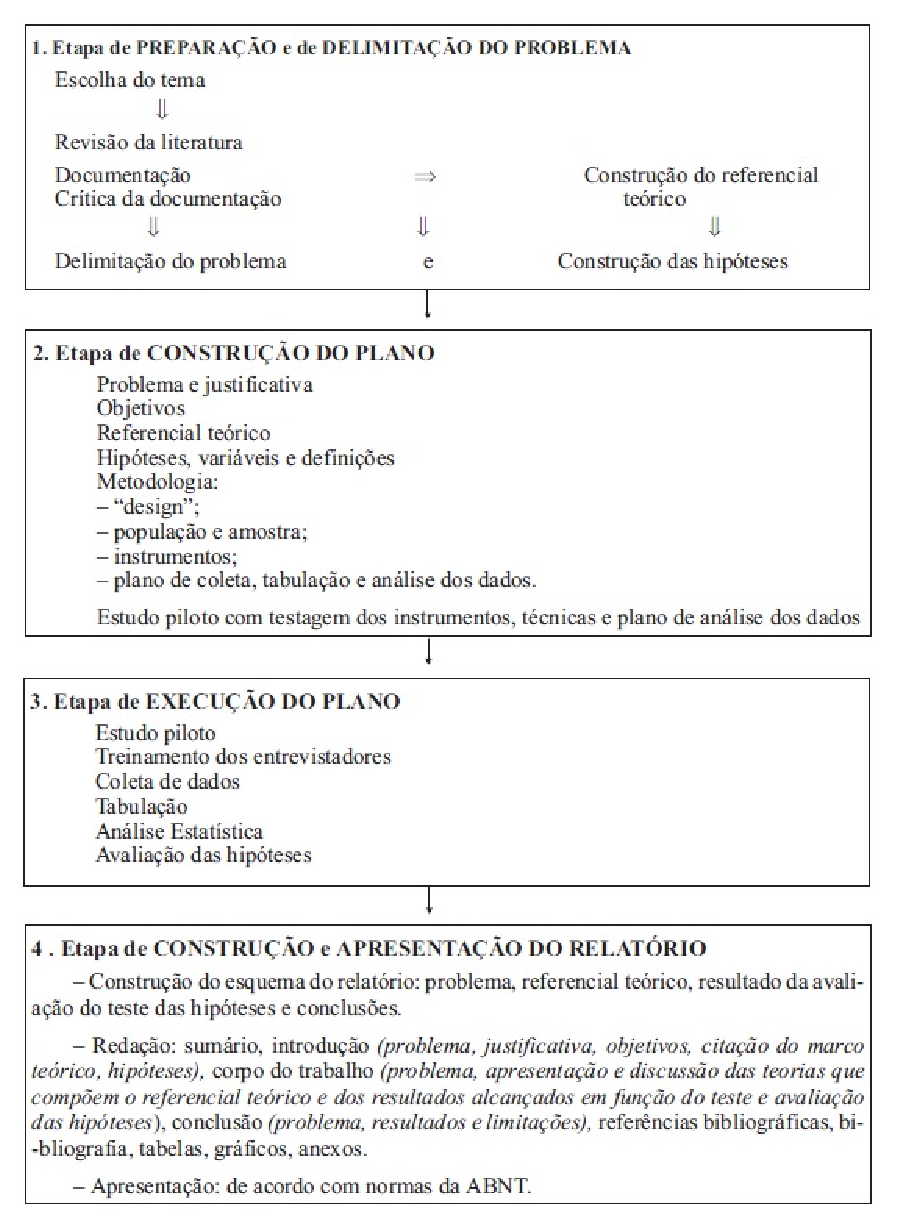
\includegraphics[keepaspectratio=true,scale=0.75]
                                      {figuras/figura18.eps}
                \caption[Fluxograma de elaboração de uma pesquisa científica]{Fluxograma de elaboração de uma pesquisa científica
                \protect\linebreak Fonte: \citeonline{koche1997}}
                \label{figura18}
    \end{figure}

    Nesse capítulo será abordado a maneira o qual foi realizada pesquisa neste projeto, o instrumento utilizado para coleta
    de dados, o cenário e os sujeitos participantes da investigação. Bem como teremos a apresentação do processso
    definido que foi utilizado na evolução deste projeto juntamente ao cronograma para acompanhamento das atividades.

    \section{Definindo a Pesquisa Científica}

        Para realizar a aplicação da Metodologia, foi necessário fazer um estudo prévio sobre o tipo de metodologia que deseja
        aplicar. Para isso é preciso conhecer cientificamente um ou mais aspectos do assunto em questão antes de avaliar qual a
        pesquisa que se deseja aplicar \cite{prodanov2013}. O produto derivado da pesquisa deverá ter cunho de contribuição para alguma área, de
        modo a afetar os envolvidos, no caso o objetivo estabelecido de tentar alcançar um patamar de processamento mais
        rápido que irá ajudar a empresa alvo.

        A figura \ref{figura19} apresenta um processo para inferir o tipo de pesquisa cientifica que se deseja realizar, e foi com
        base nesse fluxo e dentre outras atribuições, que foi possível chegar a um modelo geral de pesquisa cientifica que atende
        ao processo deste trabalho, como pode ser visto na figura \ref{figura20}.

        \begin{figure}[ht!]
        \centering
            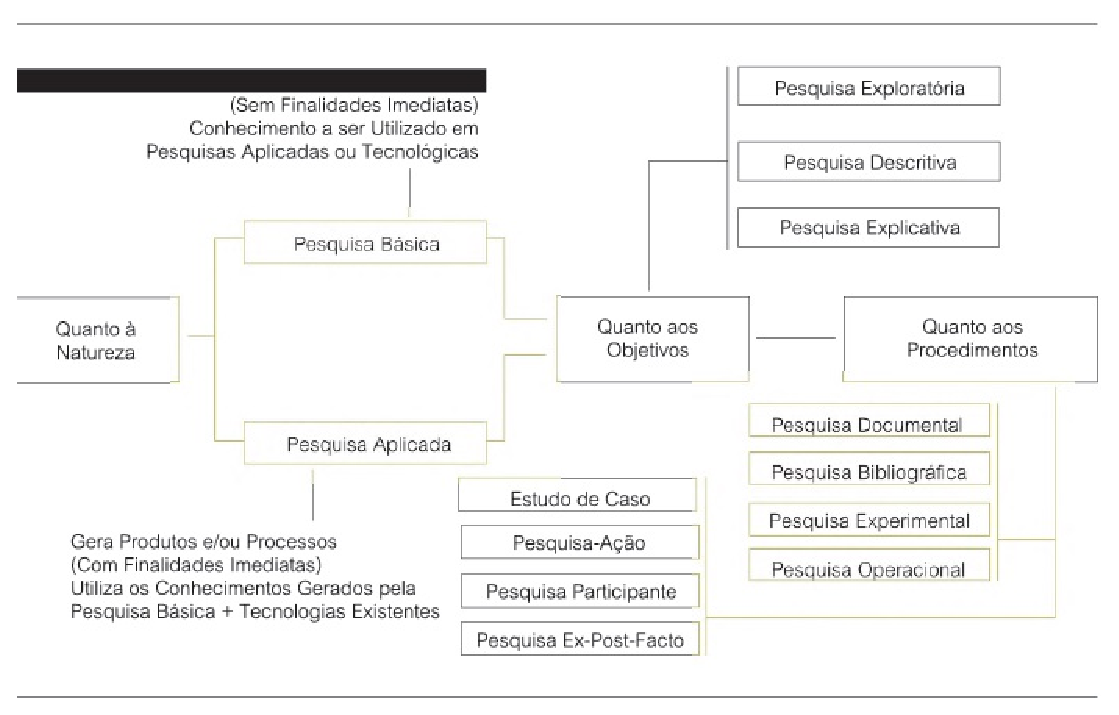
\includegraphics[keepaspectratio=true,scale=0.65]
                                      {figuras/figura19.eps}
                \caption[Tipos de Pesquisa Científica]{Tipos de Pesquisa Científica
                \protect\linebreak Fonte: \citeonline{prodanov2013}}
                \label{figura19}
        \end{figure}

        \begin{figure}[ht!]
        \centering
            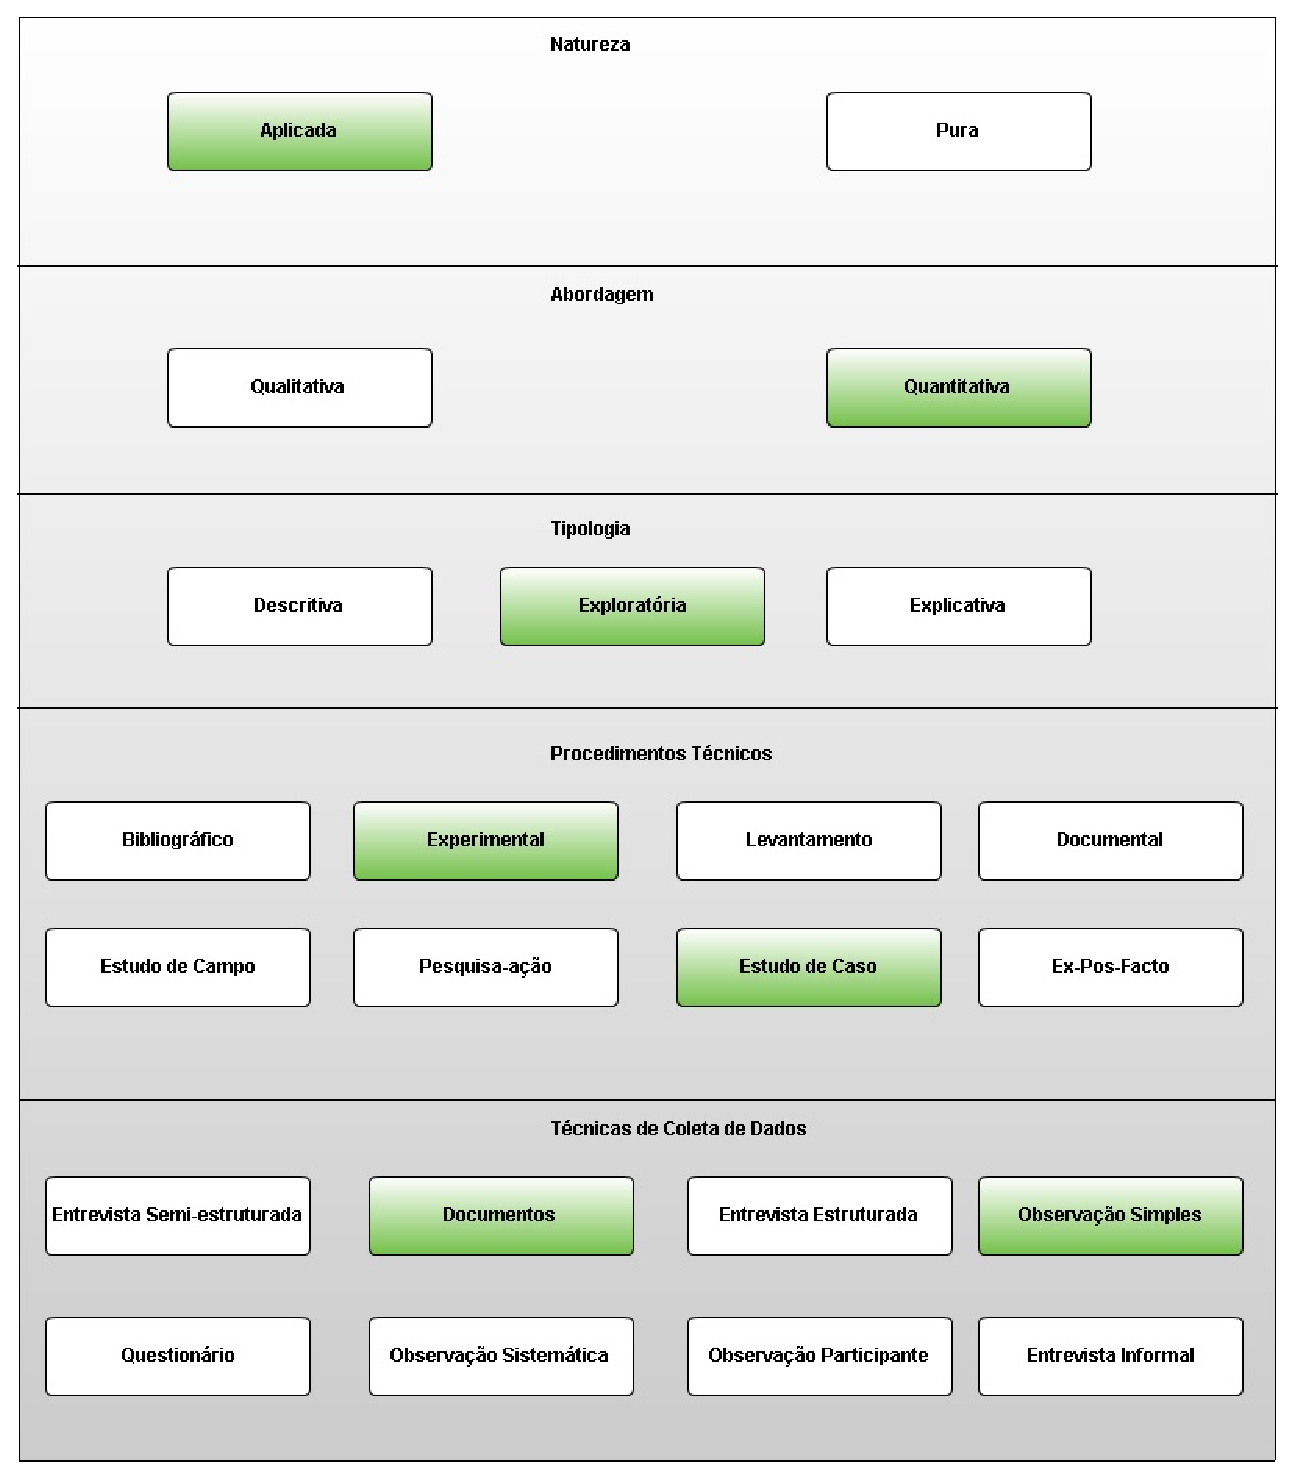
\includegraphics[keepaspectratio=true,scale=0.5]
                                      {figuras/figura20.eps}
                \caption[Metodologia de Pesquisa adotada no Trabalho]{Metodologia de Pesquisa adotada no Trabalho
                \protect\linebreak Fonte: Autor}
                \label{figura20}
        \end{figure}

        A Natureza de uma pesquisa se compreende ao contexto em que a pesquisa irá se dirigir, pois a natureza pode gerar uma
        pesquisa de objetivo básico que envolve verdade e interesse universais ou pode ser aplicada que envolve interesses e
        verdades locais \cite{lakatos2010}.

        A abordagem da pesquisa define se a pesquisa terá um cunho mais objetivo ou subjetivo ou ambos. Dependendo do tipo de
        abordagem que for adotada, diferentes técnicas serão aplicadas. A definição da abordagem tem uma importância para saber
        se o pesquisador deseja por exemplo refutar uma hipótese usando dados empíricos ou talvez trazer um entendimento
        subjetivo a uma determinada afirmação que ainda não está clara, em um determinado contexto \cite{prodanov2013}.

        O objeto de estudo está ligado a tipologia definida no processo de pesquisa cientifica. O objeto de estudo será o alvo da
        pesquisa e a tipologia será como será feito o controle da abordagem. A tipologia também a aliada aos procedimentos
        técnicos que serão realizados e das técnicas de coleta de dados que serão utilizadas \cite{prodanov2013}.

        Os procedimentos técnicos será a maneira que o pesquisador irá utilizar para obter os dados necessários para realizar a
        pesquisa. Para isso existe uma necessidade de realização de um modelo conceitual e operativo, basicamente a definição
        de um processo pelo qual o dado irá passar, ou seja, o tratamento que irá ser realizado para derivar a sua informação,
        dentro do conjunto e contexto o qual estão aplicados \cite{lakatos2010}.

        Aliado aos procedimentos técnicos, os pesquisadores também precisam escolher as técnicas de coleta de dados, que serão
        os locais aonde serão armazenados os dados extraídos bem como as informações que serão derivadas. É um lugar
        para se manter o controle dos dados que regem a base do trabalho, que serão alvos de análises para derivar as informações
        que se desejam encontrar \cite{prodanov2013}.

        E agora será explicado cada ponto escolhido da metodologia na pesquisa cientifica, que serão utilizados na abordagem do trabalho:

        \begin{itemize}
            \item \textbf{Natureza Aplicada:} Tem o objetivo de gerar conhecimentos para uma determinada aplicação prática, e
                                                                    são voltados à uma solução de problemas específicos. Envolve verdades e interesses
                                                                    locais \cite{prodanov2013}.
            \item \textbf{Abordagem Quantitativa:} Esta abordagem é uma abordagem que considera que todos os fatores na pesquisa
                                                                              podem ser quantificáveis, ou sejam tradução para números exatos. Quando existe
                                                                              uma busca pela relação de causa-efeito entre variáveis, bem como a facilidade de
                                                                              descrição da complexidade de determinados fatos ou de um problema, ou a análise
                                                                              de interação de certas variáveis, a compreensão e classificação dos dados comparados,
                                                                              são ações que a abordagem quantitativa permite responder sem a subjetividade estar
                                                                              envolvida \cite{prodanov2013}.
            \item \textbf{Tipologia Exploratória:} Apesar da tipologia exploratória, a finalidade de proporcionar mais informações sobre
                                                                          assunto, vai além disso, irá incluir a investigações de variáveis, o delineamento do
                                                                          sistema, a delimitação do escopo. Essa abordagem de tipologia exploratória irá ser
                                                                          aplicada de forma mais aprofundada com o objetivo de achar quais as variáveis que
                                                                          regem uma determinada ação do sistema (objeto de estudo) \cite{prodanov2013}.
            \item \textbf{Procedimento Técnico Experimental:} Após determinar o objeto de estudo, serão avaliadas as variáveis que
                                                                                                 o influenciam, e para isso existe uma necessidade de controle a
                                                                                                 observação dos efeitos que essas variáveis produzem no objeto. O
                                                                                                 objetivo é tentar refazer as condições de um fato a ser estudado, para
                                                                                                 observação e controle, no caso realizar o processamento de dados que a
                                                                                                 empresa realizou em cima dos dados que foram abordados \cite{lakatos2010}. A
                                                                                                 manipulação dessas variáveis irá proporcionar ao estudo, uma relação
                                                                                                 entre causa e efeito no objeto de estudo, e com base nessa relação que
                                                                                                 este projeto irá buscar aprofundar as análises para averiguar o resultado
                                                                                                 do efeito com base na observação dessas variáveis e o impacto delas
                                                                                                 no sistema \cite{prodanov2013}.
            \item \textbf{Procedimento Técnico Estudo de Caso:} O estudo de caso consiste em coletar e analisar informações sobre o
                                                                                                    objeto de estudo a fim de entender os aspectos variados que regem
                                                                                                    seu comportamento, com base no assunto da pesquisa. É um tipo de
                                                                                                    pesquisa qualitativa e ou quantitativa, entendido como uma categoria
                                                                                                    de investigação que tem como objeto o estudo de uma unidade de
                                                                                                    forma aprofundada \cite{gil2010}. Neste tipo de abordagem existem algumas
                                                                                                    limitações que podem atrapalhar a realização da pesquisa como:
                                                                                                    falta de rigor metodológico, dificuldade de generalização e tempo
                                                                                                    destinado à pesquisa. E a escolha deste procedimento técnico é
                                                                                                    importante por que no contexto em que este projeto se encontra,
                                                                                                    trata-se de um estudo de caso que está em andamento \cite{prodanov2013}.
            \item \textbf{Técnica de Coleta de Dados Documental:} A coleta de dados a ser realizada será por um repositório de dados,
                                                                                                        onde cada arquivo da análise será tratado como documento, esse
                                                                                                        tipo de armazenamento de dado será utilizado por toda base de
                                                                                                        dados bem como as análises.
            \item \textbf{Técnica de Coleta de Dados Observação Simples:} É empregada em estudos exploratórios e não tem
                                                                                                                      planejamento e controle realizados. A utilização desta
                                                                                                                      técnica vai depender do pesquisador bem como em
                                                                                                                      comparação com os dados obtidos e guardados nos
                                                                                                                      documentos. Esta técnica consiste em recolher e registrar
                                                                                                                      os fatos que estão sendo observados, no caso a
                                                                                                                      observação das métricas de precisão que irão indicar
                                                                                                                      se o sistema indo de acordo com o esperado ou não,
                                                                                                                      na velocidade do processamento dos dados \cite{prodanov2013}.
        \end{itemize}

    \section{Processo e Cronograma da Pesquisa}

        Foi realizada uma modelagem de todo o processo deste trabalho. O objetivo é ter uma visão de como o trabalho irá ser
        organizar ao longo do tempo, e com a complementação do cronograma, será possível ter uma visualização macro e micro
        das atividades que são realizadas ao longo da realização deste trabalho. Na figura \ref{figura21} e \ref{figura22} são
        apresentados os processos que regem este trabalho.

        \begin{figure}[ht!]
        \centering
            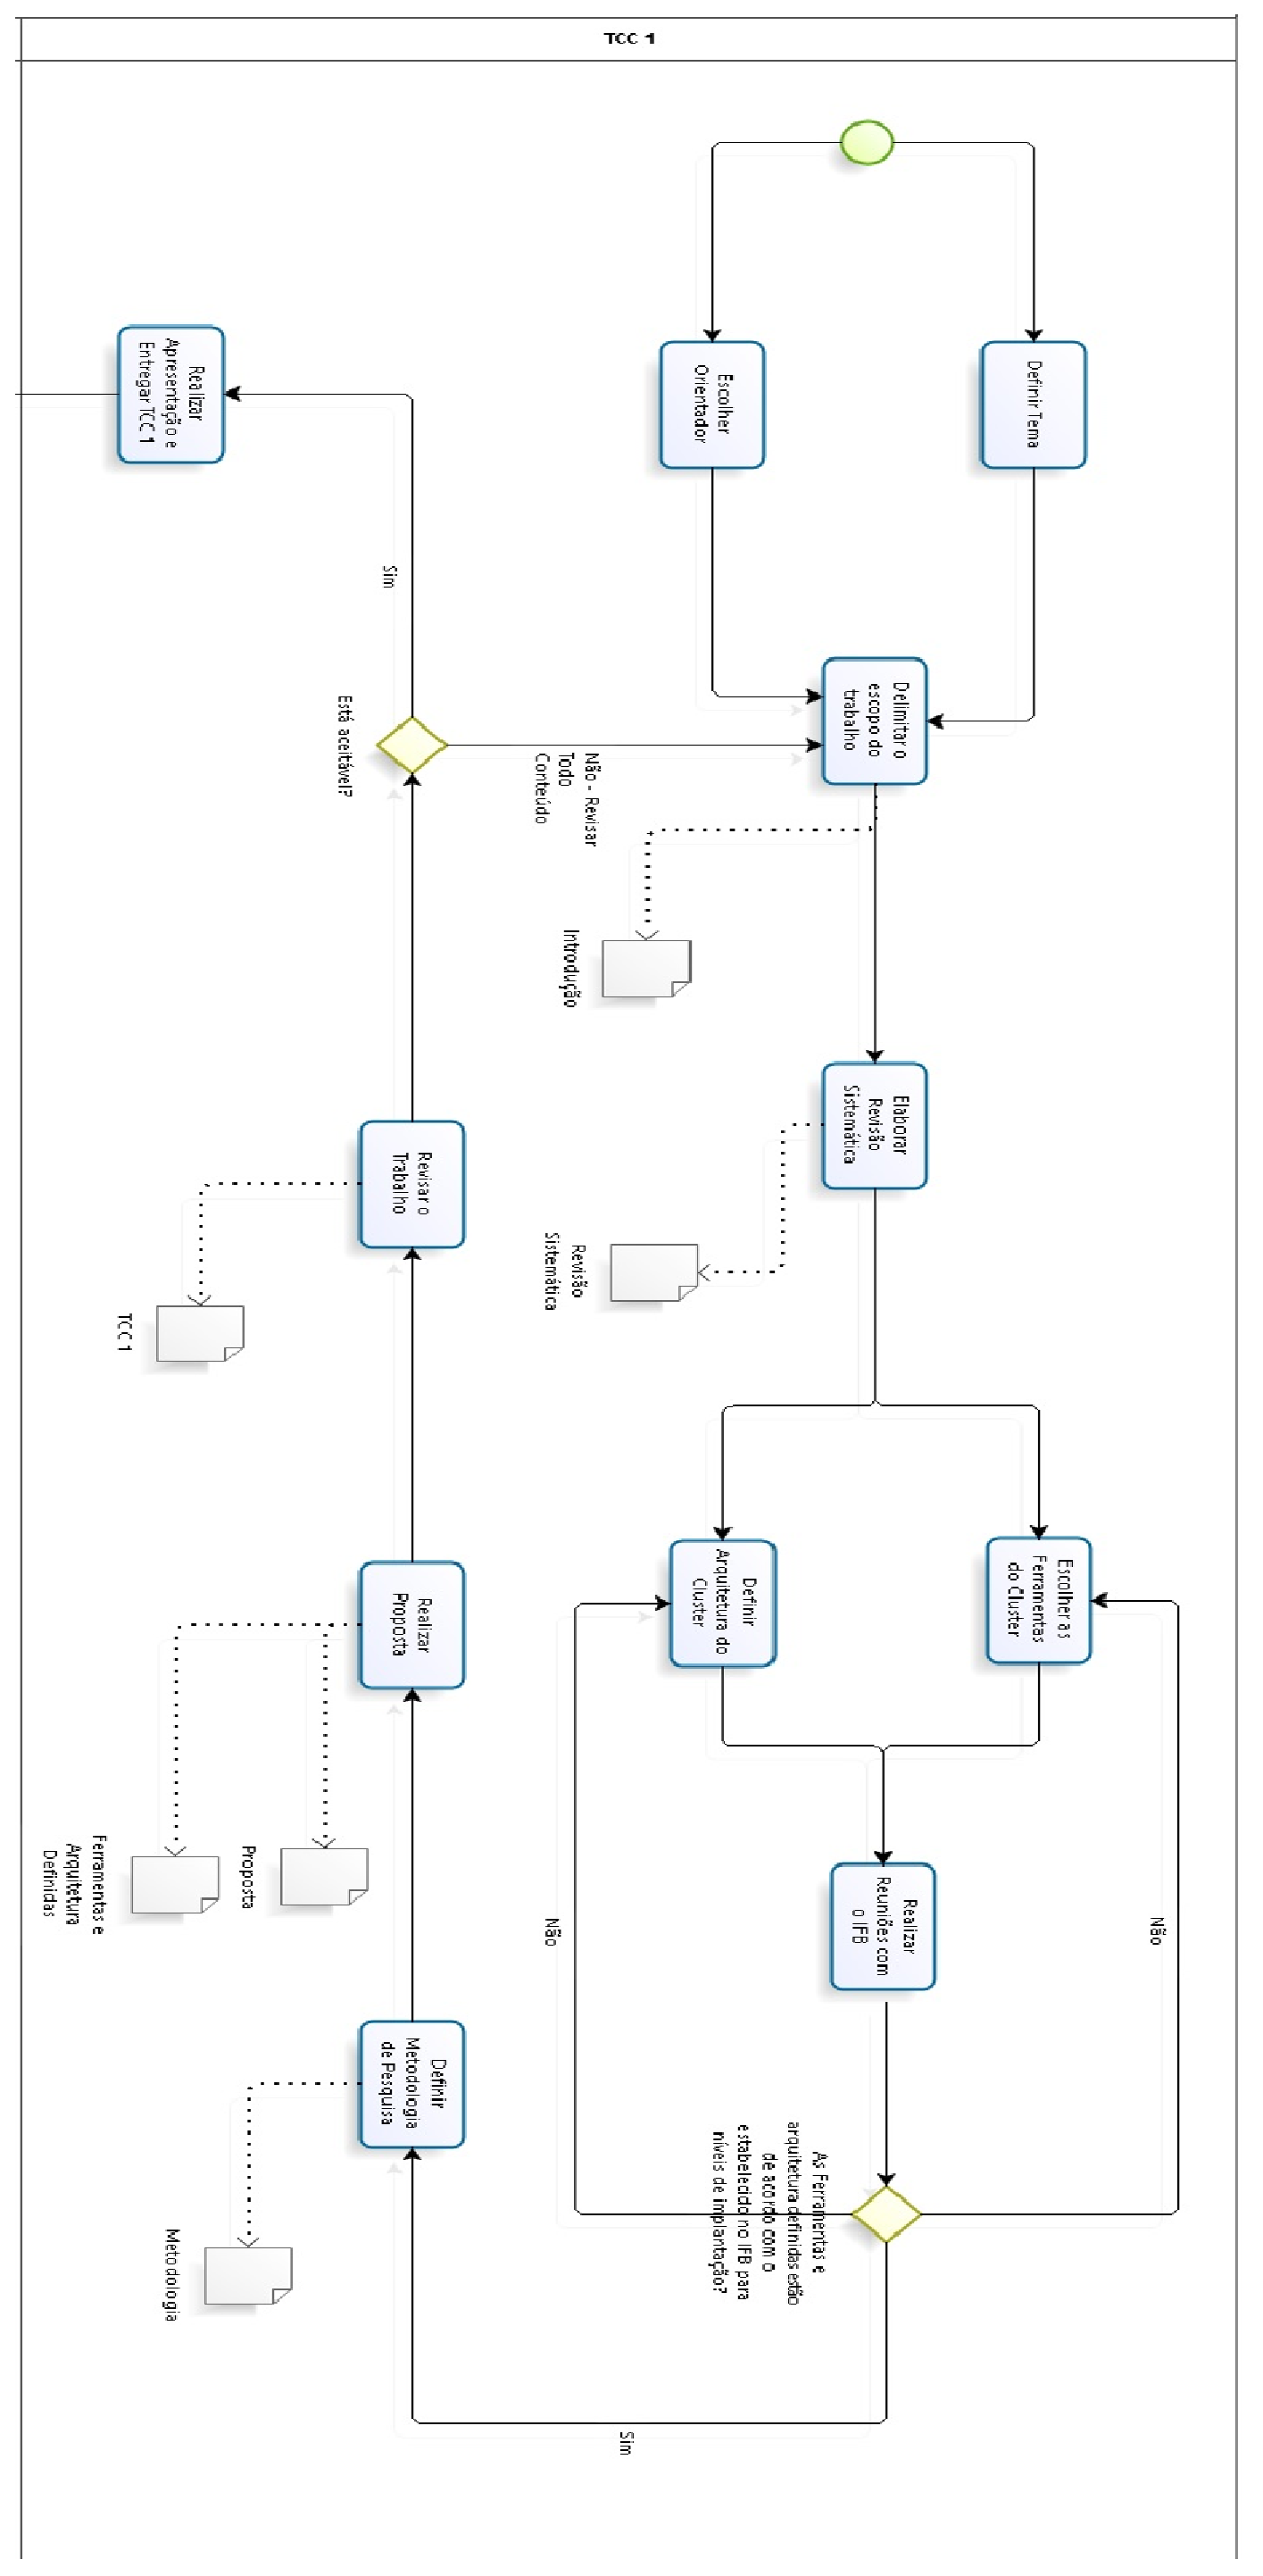
\includegraphics[keepaspectratio=true,scale=0.5]
                                      {figuras/figura21.eps}
                \caption[Processo do TCC 1]{Processo do TCC 1 -
                \protect Fonte: Autor}
                \label{figura21}
        \end{figure}

        \begin{figure}[ht!]
        \centering
            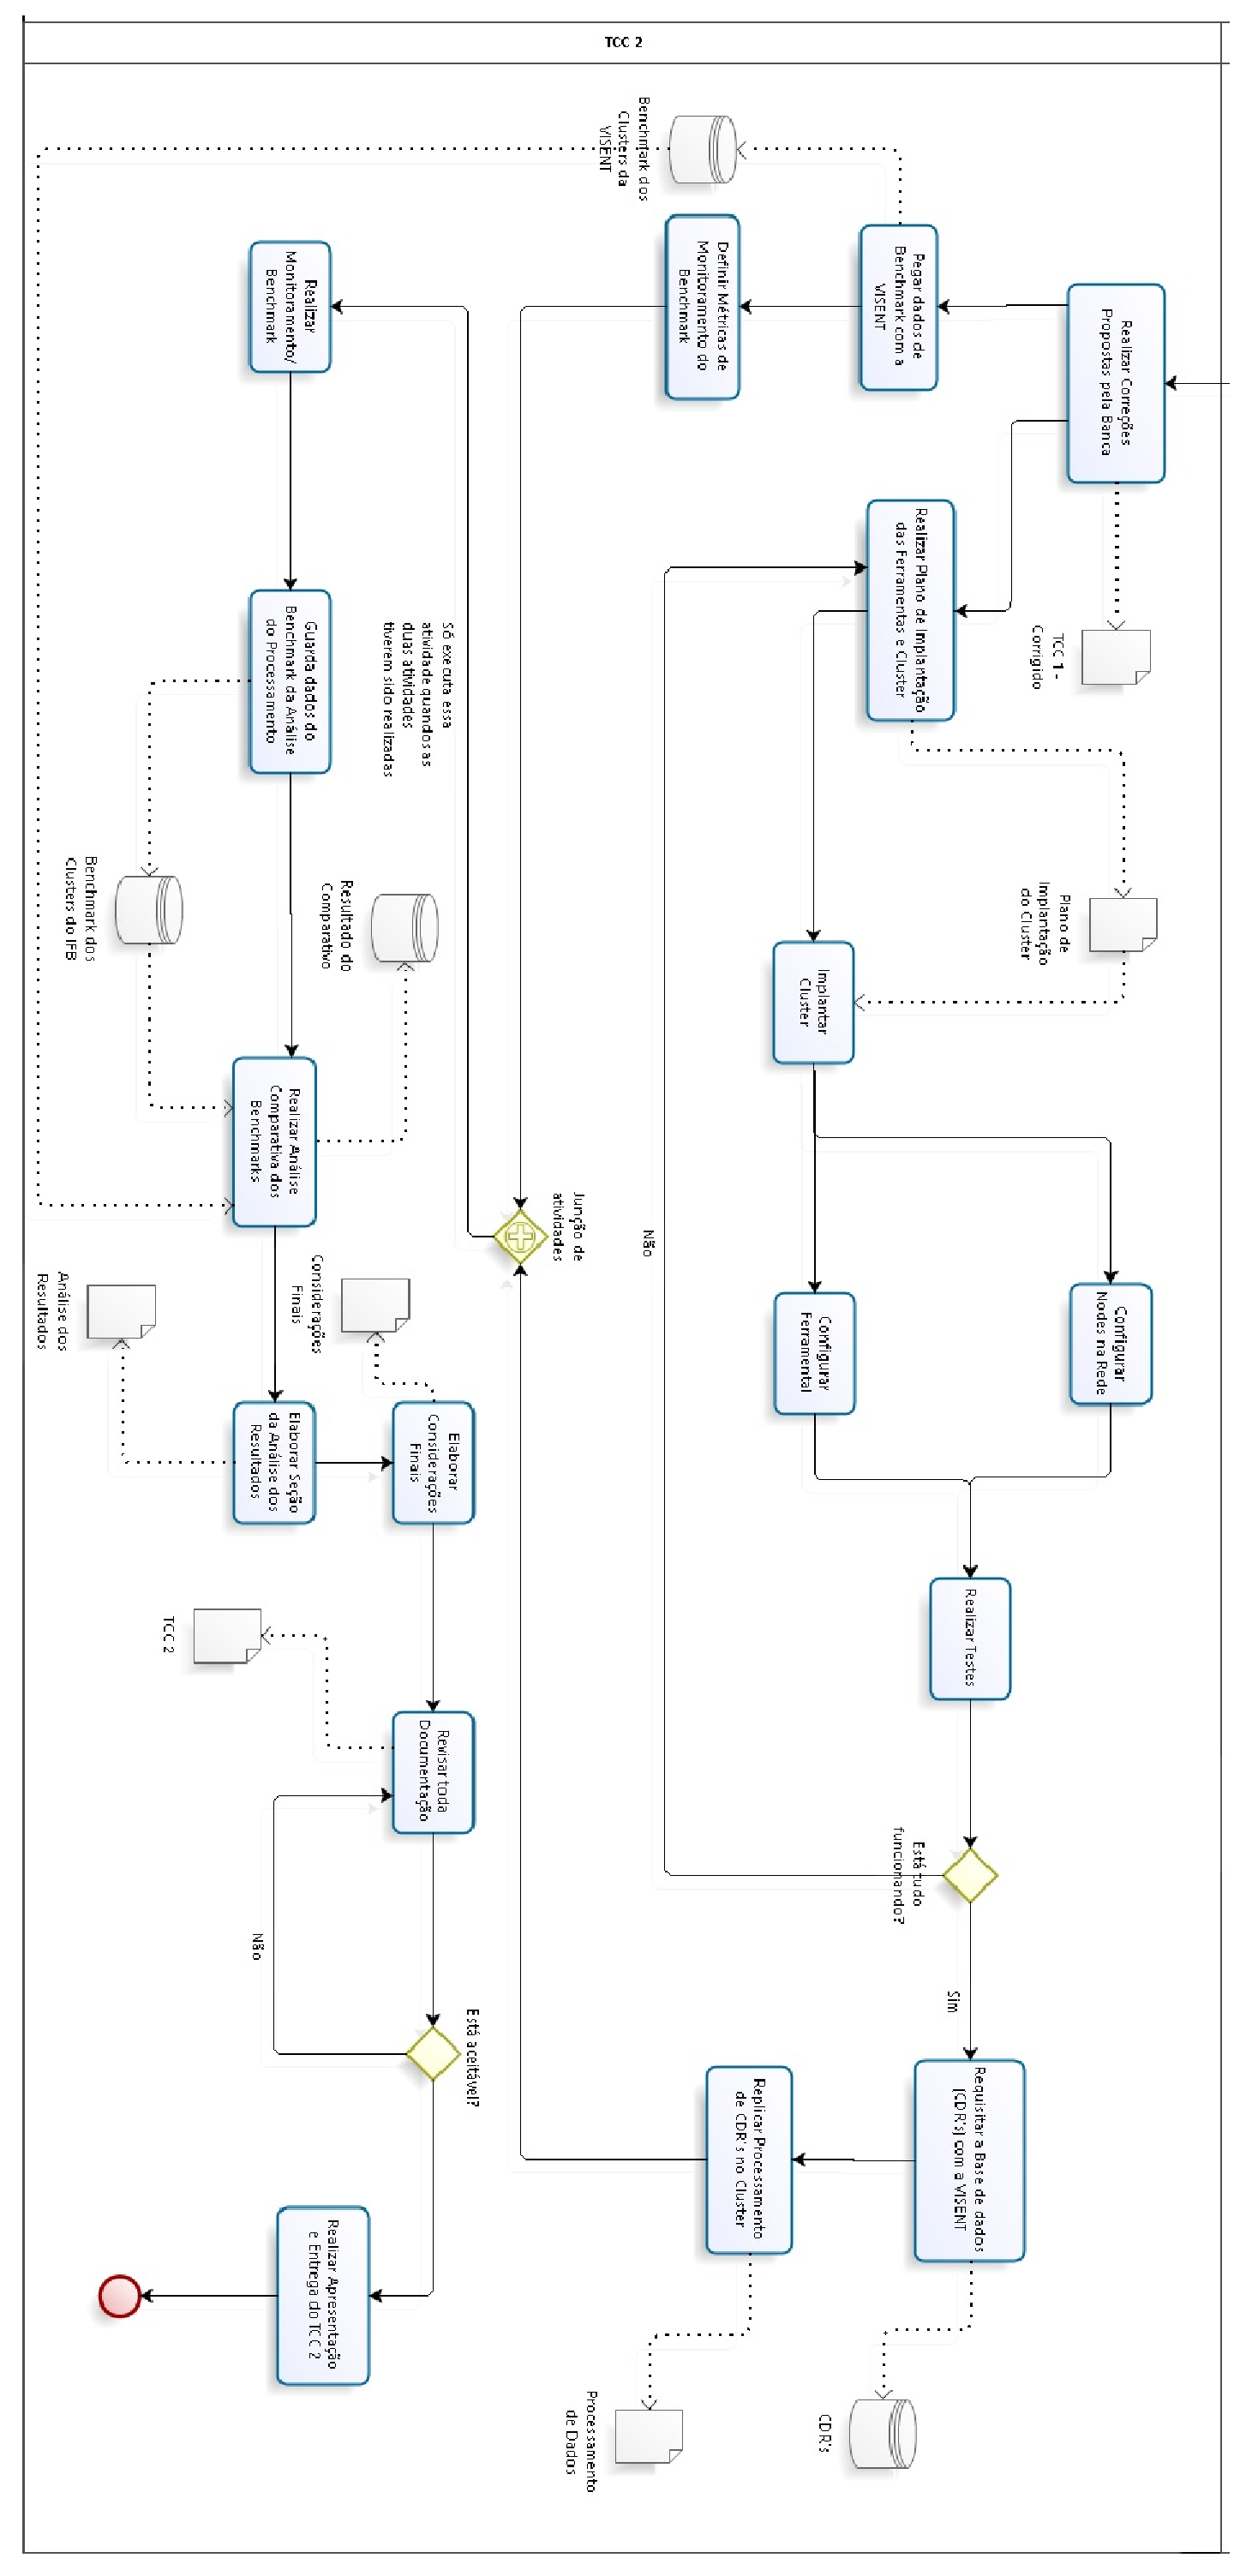
\includegraphics[keepaspectratio=true,scale=0.5]
                                      {figuras/figura22.eps}
                \caption[Processo do TCC 2]{Processo do TCC 2 -
                \protect Fonte: Autor}
                \label{figura22}
        \end{figure}

        E agora por fim nas tabelas \ref{tabela4} e \ref{tabela5}, é apresentado um respaldo geral no cronograma, sobre as
        atividades que estão sendo realizadas e que serão realizadas:

        \begin{table}[!ht]
            \begin{center}
              \begin{tabular}{|p{8cm}|p{1.3cm}|p{1.5cm}|p{1cm}|p{1cm}|p{1cm}|p{1cm}|}
                \hline
                \centering{Atividades} & Janeiro & Fevereiro & Março & Abril & Maio & Junho
                \\ \hline
                \textit{Realizar Estudo do Referencial Teórico} & x & x & x & x & &
                \\ \hline
                \textit{Delimitar Escopo e Elaborara Introdução}& & & x & x & &
                \\ \hline
                \textit{Escolher as Ferramentas} & & & x & x & x &
                \\ \hline
                \textit{Definir a Arquitetura do Cluster} & & & & x & x &
                \\ \hline
                \textit{Realizar Reuniões com o IFB} & & & & x & x &
                \\ \hline
                \textit{Definir Metodologia de Pesquisa} & & & & & x & x
                \\ \hline
                \textit{Delimitar e Elaborar Proposta} & & & & & x & x
                \\ \hline
                \textit{Revisar TCC 1} & & & & & & x
                \\ \hline
              \end{tabular}
              \caption[Cronograma TCC 1]{Cronograma TCC 1
              \protect \linebreak Fonte: Autor}
            \label{tabela4}
            \end{center}
        \end{table}

        \begin{table}[!ht]
            \begin{center}
              \begin{tabular}{|p{7cm}|p{1cm}|p{1.1cm}|p{1.5cm}|p{1.5cm}|p{1.7cm}|p{1.7cm}|}
                \hline
                \centering{Atividades} & Julho & Agosto & Setembro & Outubro & Novembro & Dezembro
                \\ \hline
                \textit{Realizar Correções no TCC} & x & x & & & &
                \\ \hline
                \textit{Realizar Plano de Implantação}& x & x & x & & &
                \\ \hline
                \textit{Implantar o Cluster} & & & x & x & x &
                \\ \hline
                \textit{Pegar dados de Benchmark da Visent} & & x & x & & &
                \\ \hline
                \textit{Configurar Nodes na Rede} & & & x & x & x &
                \\ \hline
                \textit{Configurar Ferramental} & & & x & x & x &
                \\ \hline
                \textit{Realizar Testes} & & & x & x & x &
                \\ \hline
                \textit{Requisitar a Base de Dados dos CDR's} & & x & x & & &
                \\ \hline
                \textit{Replicar Processamento de CDR's} & & & x & x & x & x
                \\ \hline
                \textit{Realizar Monitoramento/ Benchmark} & & & x & x & x & x
                \\ \hline
                \textit{Realizar Análise Comparativa dos Benchmarks} & & & & x & x &
                \\ \hline
                \textit{Elaborar Análise dos Resultados} & & & & & x & x
                \\ \hline
                \textit{Elaborar Considerações Finais} & & & & & x & x
                \\ \hline
                \textit{Revisar TCC 2} & & & & & & x
                \\ \hline
              \end{tabular}
              \caption[Cronograma TCC 2]{Cronograma TCC 2
              \protect \linebreak Fonte: Autor}
            \label{tabela5}
            \end{center}
        \end{table}

    \section{Considerações Finais do Capítulo}

        Com a metodologia de pesquisa cientifica definida, juntamente ao processo e cronograma, é possível ter uma macro
        visão do que se espera do trabalho, pois esse capítulo procurou definir esses fatores importantes para que se possa
        ter um respaldo comparativo no final do trabalho entre o que foi realizado, quais foram as dificuldades encontradas
        bem como as limitações que projeto irá encontrar, sem contar de fatores que não podem ser previstos.
